\section[惯性定律]{\makebox[5em][s]{惯性定律}}\label{sec:03.01}

在上两章中,讨论了运动的描述,而没有涉及运动的原因,
没有研究不同式样的运动之间的内在联系。譬如,自由落体为什
么垂直向下做匀加速运动?行星为什么绕太阳旋转不息?自由落
体与行星旋转两者之间有什么关系?这些就是本章及随后几章要
讨论的问题。

研究物体运动的原因,通常称之为动力学。牛顿动力学就是
有关物体的机械运动的动力学。可以说整个物理学的基本规律就
是各种运动形态的动力学的总合。

牛顿动力学中的核心概念是力。

经验告诉我们,物体的运动是由物体之间的相互作用引起的。
列车的行进是由于机车的牵引作用,枪弹的射击是靠着炸药爆炸
的作用。物体之间的相互作用,用“力”这个概念来表达。实际
上,人对力最初的认识是源于人的肌肉对外物的作用。汉字的力,
在篆书中的写法,就是筋肉的象形。

力的概念虽然出现得很早,但是关于力和运动的关系的正确
认识,却得到得相当晚。在亚里士多德的《物理学》中有一条原
理:“凡运动着的事物必然都有推动者在推动着它运动。”这个
论断在几乎两千年的时间里,被认为是无可怀疑的经典。的确,
% 090.jpg
我们日常看到的各种运动似乎都遵从这个论断,即必定有推动者
(即力)在维持着它的运动。就象一定的踏力保持着自行车的一定
的运动状态,而一当踏力消失,车最终要变成静止。

\begin{wrapfigure}[7]{r}{16.5em}
  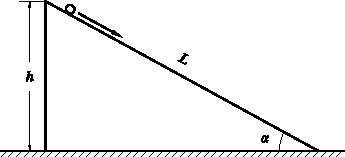
\includegraphics{figure/fig03.01}
  \caption{伽利略的斜面}
  \label{fig:03.01}
\end{wrapfigure}
伽利略开始明确地认识到亚里士多德的经典是不完全正确的,尽
管许多运动的确都要靠外力的维持,但并非凡运动皆如此。伽利略用
一个理想实验来证明亚里士多德的错误。他研究斜面上的运动(图\ref{fig:03.01}),
让一小球从斜面
上滚下。已经知道,小球的下滚是由于重力的作用,重力沿着斜面
的分量拉着小球下滚。如果高度不变,$\alpha$越小,则$ L $越大,同时
重力沿斜面的分量也越小。伽利略曾做过一系列小球沿斜面下滑
的实验。他发现,只要斜面足够光滑,无论$\alpha$多么小,小球总能
从斜面上滚下来。由这个结果就可以推测,即使当$ a \rightarrow 0$  ,$L \rightarrow \infty$
的情况,小球还是可以滚“下”来的。显然,对$ a \rightarrow 0$  ,$L \rightarrow \infty$情
况是无法直接做实验的,但从已知的实验结果可以推知这种极限
情况的现象。这就是理想实验方法的关键。

在$ a \rightarrow 0$  ,$L \rightarrow \infty$情况,重力沿斜面的分量为零,即并没有外
力推动小球“下”滚。因此,这种运动就是一种没有“推动者”
的运动。对亚里士多德的“凡运动必有推动者”来说,上述运动
就是一个反例。

伽利略的分析弄清了,存在一类运动,它们并不是由外力所
维持。它们的特征是速度保持不变,即作匀速率的直线运动,或
者静止。我们称物体不受外力作用的运动状态为自由运动。总之,
处在自由运动状态的物体,必定作匀速直线运动,或者静止。这
就是惯性定律。
% 091.jpg

有人可能会想到,速度或加速度都是具有相对性的,对参考
系$K$为匀速运动的物体,在参考系$K'$中可能成为非匀速的。那么,
一个自由运动的物体,在有些参考系看来不也是作着非匀速运动
吗?的确,在某参考系看来,一个不受力的物体也会作非匀速运
动。

然而,惯性定律的意义是在于断言:对于一个物体的自由运
动,一定可以选择一个参考系$K$,相对于$K$该物体作匀速运动或
静止,而且,其他所有自由运动的物体,对于$K$来说,也都是作
匀速运动或静止。换言之,一定存在着这样的参考系,相对于
它,所有不受外力作用的物体都保持自己的速度。这类特殊的参
考系,称为惯性参考系,或惯性系。

简言之,惯性定律就是断定了惯性系一定存在。

惯性定律的确立,成为旧物理学(即亚里士多德物理学)的终
点,同时也成为新的力学的起点。常称惯性定律为牛顿第一定律。
本章以后的讨论,都采用惯性系。